\FloatBarrier

\begin{figure}[h!]
	\centering
	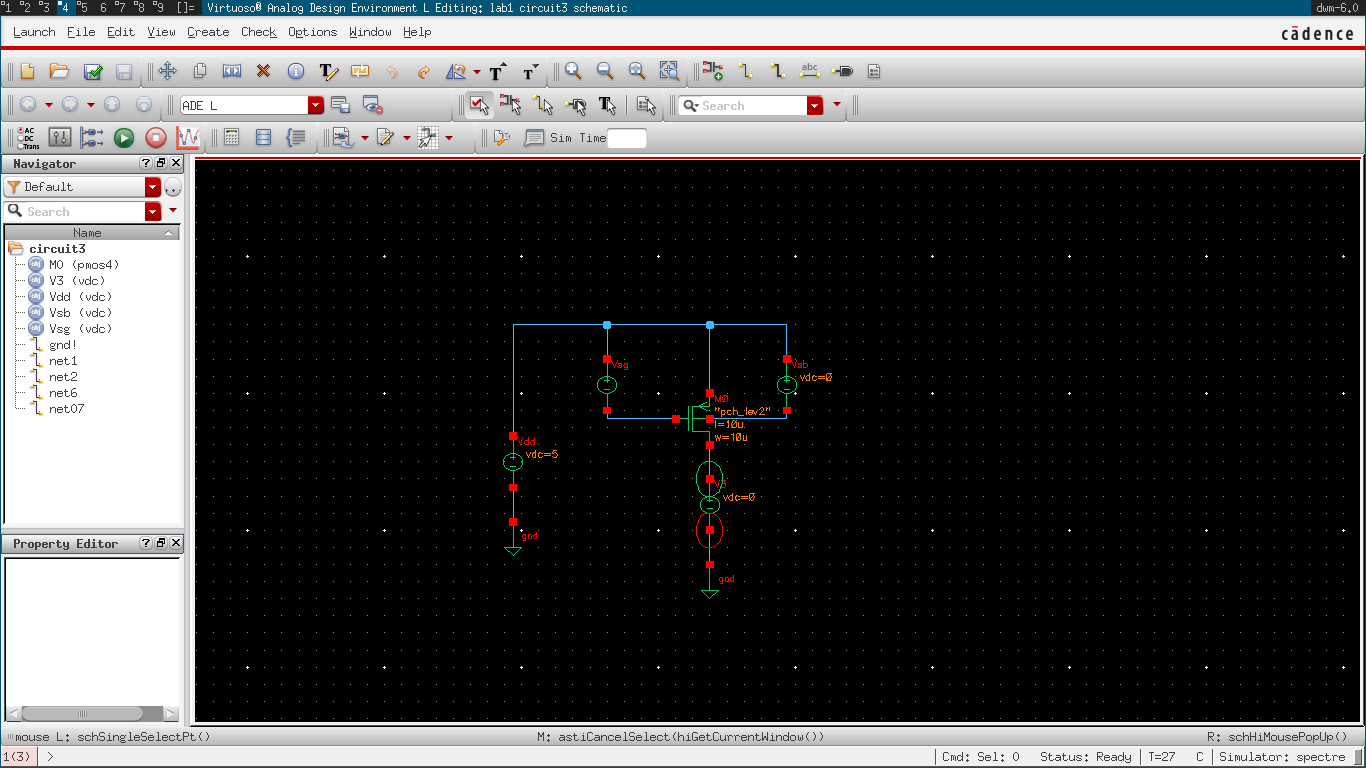
\includegraphics[scale=0.75]{../images/circuit3.PNG}
	\caption{Circuit for Simulation 3}
	\label{fig:circuit3}
\end{figure}

\FloatBarrier

Simulation 3 is similar to Simulation 1 except that a PMOS is used instead of an NMOS.

\FloatBarrier

\begin{figure}[h!]
	\centering
	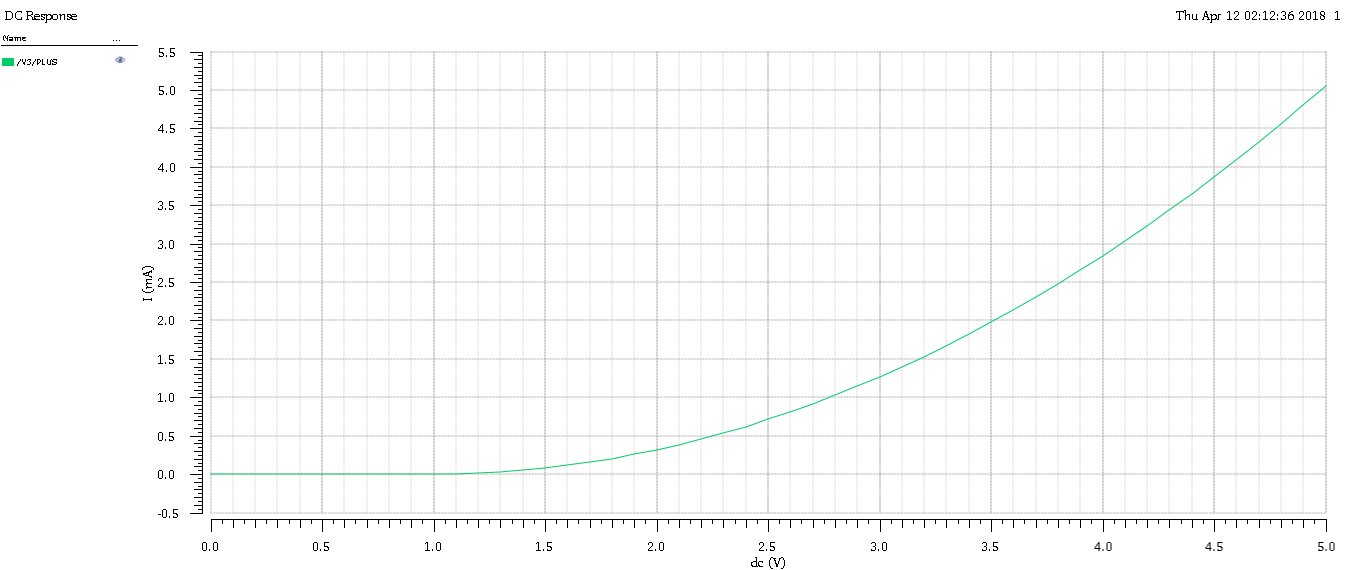
\includegraphics[scale=0.75]{../images/id_vs_vgs_pmos.PNG}
	\caption{$I_{D}$ versus $V_{GS}$ for PMOS}
	\label{fig:id_vs_vgs_pmos}
\end{figure}

\FloatBarrier

\FloatBarrier

\begin{figure}[h!]
	\centering
	\includegraphics[scale=0.75]{../images/did_vs_vgs_pmos.PNG}
	\caption{$\frac{I_{D}}{V_{SG}}$ versus $V_{SG}$ for PMOS}
	\label{fig:did_vs_vgs_pmos}
\end{figure}

\FloatBarrier

\FloatBarrier

\begin{table}[h!]
	\centering
	\caption{Simulation 3 Results}
	\label{tab:sim3_results}
	\csvautotabular{../tables/sim3_results.csv}
\end{table}

\FloatBarrier
